A fundamental issue in reinforcement learning algorithms is how to balance between exploration of the environment and exploitation of information already obtained by the agent. There is a large body of literature on efficient exploration tackling the exploration vs exploitation dilemma. The goal of exploration strategies is minimizing learning time while providing some guarantees on the performance of the learned policy. Clearly, the more effectively and efficiently an agent explores and learns from its environment, the more effectively and efficiently it uses its time, and hence, the less time is required for learning. Intuitively, one might infer that pure exploration during learning would be the most effective learning approach. However, this is not the case. Pure exploration may waste much time and computing resources exploring task-irrelevant parts of the environment. This also means that the agent's performance during learning will be poor, relatively speaking, since it spends some unnecessary portion of its time performing actions that do not help it in achieving its goals. \par
It is often advantageous to find some suitable balance of both exploration and exploitation. If the agent can exploit its current knowledge of the environment, it may be able to identify the most worthwhile parts of the environment to explore. Further, minimizing the learning costs (\ie maximizing the agent's performance during learning) cannot be done without some degree of exploration of the environment such that effective behaviours can be discovered. 
Another problem that may arise is the applicability of the exploration strategy to the task at hand. An exploration strategy that performs well in one environment may be ill suited to another environment. Thrun in ~\cite{Thrun92efficientexploration} observed that the impact of the exploration technique on both learning time and learning costs can be enormous. \par
The purpose of this chapter is to review some relevant algorithms in the field of efficient exploration, starting from the classical ones to the more modern ones. In Section ~\ref{exploration} reviews measures of efficient exploration and some algorithms that give theoretical guarantees. Section ~\ref{deep_exploration} describes deep exploration and Bootstrapped DQN as an example algorithm that performs deep exploration. Finally, Section ~\ref{distributional_rl} is devoted to algorithms that perform exploration using the value distribution, and the distributional Bellman operator.
\section{Exploration} \label{exploration}
\subsection{Measuring Efficient Exploration}
Before reviewing the state of the art in exploration, it is important to discuss how to measure the efficiency of an RL algorithm in formal terms. In this section we will review two important measures, \emph{sample complexity} and \emph{regret}.
\subsubsection{Sample Complexity}
Sample complexity defined as the time required by the algorithm to find an approximately optimal policy ~\cite{Gatsby2003OnTS}. More formally:
\begin{itemize}
 \item Let $\mathcal{M}$ be an MDP with N states, K actions, discount factor $\gamma$ and a maximal reward $R_{max}$ >0;
 \item Let A be an algorithm that acts in the environment producing experience $s_0$, $a_0$, $r_1$, $s_1$, $a_1$, $r_2$ $\ldots$;
 \item Let $V^{A}_t=\mathbb{E} \left[ \sum_{\tau =0}^{\infty} \gamma^\tau r_{t+\tau} \mid s_0,a_0,r_1 \ldots s_{t-1},a_{t-1},r_t,s_t \right]$ be the value accumulated by A;
 \item Let $V^*$ be the value function of the optimal policy;
\end{itemize}
\begin{definition}
	Let $\epsilon > 0 $ be a prescribed accuracy and $\delta > 0$ be an allowed probability of failure. The expression $\eta(\epsilon,\delta,N,K,\gamma,R_{max})$ is a sample complexity bound for algorithm A if independently of the choice of $s_0$,with probability at least $1-\delta$, the time steps such that $V^{A}_t < V^* - \epsilon$ is at most $\eta(\epsilon,\delta,N,K,\gamma,R_{max})$.
\end{definition}
Now that we have a measure of the efficiency of RL algorithms, we can give the definition of \emph{PAC-MDPs}, a class of algorithms which includes some of the algorithms we will discuss further.
\begin{definition}
An algorithm with sample complexity that is polynomial in $\frac{1}{\epsilon}$, $\log\frac{1}{\delta}$, $N$, $K$, $\frac{1}{1-\gamma}$, $R_{max}$ is called PAC-MDP (probably approximately correct in MDPs).
\end{definition}
\subsubsection{Regret}
Regret is defined as the difference between the cumulative reward of the optimal policy and that gathered by the policy $\pi$ played by the agent hence is usually used with on-policy algorithms. More formally, the total regret of policy $\pi$ after $T$ steps, $R^{\pi}(T)$ is defined as:
\begin{equation}
	R^{\pi}(T)=\sum_{t=1}^{T}\left(V^{\pi^*}(s_t^{\pi^*})-V^{\pi^t}(s_t^{\pi})\right),
\end{equation}
where $s_t^{\pi^*}$ is the state the agent would have been in time step $t$, if he had followed optimal policy $\pi^*$. Regret measures the cumulative reward loss due to the need of learning, quantifying the exploration vs. exploitation dilemma. 
\subsection{Explicit Explore or Exploit}
In the previous chapter we shortly reviewed the Q-Learning algorithm. An important characteristic of Q-learning is that it is a model-free approach to learning an optimal policy in an MDP with unknown parameters. In other words, there is not an explicit attempt to model or estimate costs and/or transition probabilities, the value of each action is estimated directly through samples. Another approach to the same problem is to estimate the MDP parameters from the data and find a policy based on the estimated parameters (model-based). In this sections, we will review an algorithm of that class specifically designed for efficient exploration, the Explicit Explore or Exploit ($E^3$) algorithm, proposed by Kearns and Singh ~\cite{Kearns:2002:NRL:599616.599699}. $E^3$ is a model-based, PAC-MDP algorithm which assumes knowlwdge of the maximum reward of the MDP and uses the concept of \emph{optimism in the face of uncertainty}.\par 
The main ideas of $E^3$ are as follows :
\begin{itemize}
	\item The state space $S$ is divided in two parts, \emph{known states} $N$ and \emph{unknown states} $N^C$,
	\item Counters for state and actions are kept to quantify confidence in model estimates,
	\item Known states have been visited sufficiently many times to guarantee that the transition probabilities $P(s,a,s')$ and rewards $R(s,a,s')$ are accurate with high probabilities for every tuple $(s,a,s') \in S \times A \times S$,
	\item Unknown states are moved to the known set, $N$, when they are visited at least $m$ times, for some number $m$.
\end{itemize}
By separating the state space in two subsets, $E^3$ defines two different MDPs. The first MDP, $MDP_{known}$, includes the states in the set N and the calculated values for the transition probabilities and Reward function. This MDP is used for exploitation. The second MDP, $MDP_{unknown}$, has the same structure as the first one with the addition of a special state $s'$ which includes all the unknown states and the reward for reaching it is maximal, for every action $a \in A$. Pseudocode of the $E^3$ algorithm is shown in Alg.~\ref{alg:e3}
\begin{algorithm}[H]
\begin{flushleft}
 \textbf{Input:} $s$ - Current state\\
 \textbf{Output:} $a$ -Action to execute
\end{flushleft}
 \begin{algorithmic}
 
 \If{$s$ is known }
 \State Plan in $MDP_{known}$
 \If{resulting plan has value above some threshold}
 \State \Return first action of plan
 \Else
 	 \State Plan in $MDP_{unknown}$
 	 \State \Return first action of plan
 \EndIf
 \Else
 	\State \Return action with the least observations in $s$
 \EndIf
 \end{algorithmic}
 \caption{$E^3$ algorithm}
 \label{alg:e3}
\end{algorithm}
$E^3$ makes the exploitation vs exploration dilemma explicit by choosing in which of the two MDPs to plan, based on the confidence it has on the model parameters estimated so far. Kearns and Singh ~\cite{Kearns:2002:NRL:599616.599699} show that, with probability no less than $1-\delta$, $E^3$ will stop after a number of actions and computation time $poly(\frac{1}{\epsilon},\frac{1}{\delta},N,\frac{1}{1-\alpha},R_{max})$. The number of samples required to solve the MDP is polynomial in the number of states, so the algorithm is called efficient. However, in natural environments, the number of states is enormous, exponential to the number of state variables. This makes $E^3$ exponential in the number of states variables. 
\subsection{R-Max}
R-max is a very simple model-based reinforcement learning algorithm which can attain near-optimal average reward in polynomial time. In R-max, the agent always maintains a complete, but possibly inaccurate model of its environment and acts based on the optimal policy derived from this model. The model is initialized in an optimistic fashion: all actions in all states return the maximal possible reward (hence the name). During execution, it is updated based on the agent's observations.
R-max improves upon several previous algorithms: (1) It is simpler and more general than Kearns and Singh’s $E^3$ algorithm, covering \emph{zero-sum stochastic games}. (2) It has a built-in mechanism for resolving the exploration vs. exploitation dilemma. (3) It formally justifies the \emph{optimism under uncertainty} bias used in many RL algorithms. (4) It implicitly addresses the exploration vs exploitation dilemma.\par
\subsubsection{Stochastic Games}
Before explaining how R-max works, it is important to shortly define the framework of stochastic games. We consider a stochastic game $\mathcal{M}$ consisting of a set $\mathcal{S}= \lbrace G_1,\ldots,G_N \rbrace$ of stage-games in which both the agent and the adversary, have a set $\mathcal{A}= \lbrace a_1,\ldots,a_K \rbrace$ of possible actions. We associate a reward matrix $R^i$ with each game, and use $R^i_{m,l}$ to denote a pair consisting of the reward obtained by the agent and the adversary after playing actions $a_m$ and $a_l$ in game $G_i$, respectively. In addition, we have a probabilistic transition function, $P_M$, such that $P_M(s,t,a,a')$ is the probability of making a transition from $G_s$ to $G_t$ given that the agent played $a$ and the adversary played $a'$. This way, all model
parameters, both rewards and transitions, are associated with joint actions of a particular game.
\subsubsection{R-max algorithm}
In R-max, the agent will always attempt to optimize its behavior, albeit with respect to a fictitious model. Roughly speaking, this model assumes that the reward the agent obtains in any situation it is not too familiar with is its maximal possible reward, denoted by $R_{max}$. Often, optimal behavior with respect to this fictitious
model results in exploration with respect to the real model, and thus, to learning. The
major insight behind the R-max algorithm is that the optimal policy with respect to the agent’s fictitious model has a very interesting and useful property with respect to the real model: it is always either optimal or it leads to efficient learning. In many situations, the agent will not know ahead of time whether its behavior will lead to optimizing behavior with respect to the real model or to learning – this depends on how the adversary will act. However, it knows that it will either optimize or learn efficiently.\par
The approach taken by R-max is not new. It has been referred to as the optimism in the face of uncertainty heuristic, and was considered an ad-hoc, though useful, approach ~\cite{KLMSurvey,Sutton:1998:IRL:551283}. The approach has been extensively studied in the framework of multi armed bandits ~\cite{journals/corr/abs-1204-5721}. This optimistic bias has also been used in a number of well-known reinforcement learning algorithms, e.g. Kaelbling’s interval exploration method ~\cite{kaelbling1993learning}, the exploration bonus in Dyna ~\cite{DBLP:journals/sigart/Sutton91} etc. However, none of this work provides theoretical justification for this very natural bias. Brafman and Tennenholtz ~\cite{Brafman:2003:RGP:944919.944928} provide a formal justification for the optimism under uncertainty bias, used in their R-max algorithm.\par
The algorithm is quite simple. Model $\mathcal{M}'$ is constructed, containing the set of $N+1$ games $\mathcal{S}= \lbrace G_0,G_1,\ldots,G_N \rbrace$, where $G_0$ is an initial fictitious game, and the set of $k$ actions $\mathcal{A}= \lbrace a_1,\ldots,a_K \rbrace$. The reward matrices are initialized to have ($R_{max},0$) in all entries whereas the transition model is initialized $P_M(G_i,G_0,a,a′)$ = 1 for all i=$0,\ldots,N$ and for all actions $a,a′$. In addition, for each game, we maintain some additional information:
\begin{itemize}
\item a boolean value depicting whether the state is \emph{known} or \emph{unknown}, initiliazed to unknown;
\item the states reached by playing the joint action corresponding to this entry (and how many times each state was reached), initially empty;
\item the reward obtained (by both players) when playing the joint action
corresponding to this entry, initially empty.
\end{itemize}
The algorithm assumes knowledge of the maximum reward, $R_{max}$, and the $\epsilon$-return mixing time of an optimal policy, $T$. After the initialization phase the algorithm enters its main loop, composed of two phases. The first phase called \emph{Compute and Act}, computes an optimal $T$ -step policy for the current state, and executes it for $T$-steps or until a new entry becomes known. The second phase, \emph{Observe and update}, follows each joint action as follows: Let $a$ be the action the agent performed in $G_i$ and let $a'$ be the adversary's action:
\begin{itemize}
\item If the joint action ($a,a'$) is performed for the first time in $G_i$, update the reward associated with ($a,a'$) in $G_i$, as observed;
\item Update the set of states reached by playing ($a,a′$) in $G_i$ ;
\item If at this point your record of states reached from this entry contains \\ $K_1=\max \left( \lceil (\frac{4NTR_{max}}{\epsilon})^3 \rceil,\lceil -6 \ln^3(\frac{\delta}{6Nk^2}) \rceil \right) +1$ elements, mark this entry as known and update the transition probabilities for this entry according to the observed frequencies.
\end{itemize}
R-max starts with an initial estimate for the model parameters that assumes all states and all joint actions yield maximal reward and lead with probability 1 to the fictitious stage-game $G_0$. Based on the current model, an optimal $T$-step policy is computed and followed. Following each joint action the agent arrives at a new stage-game, and this transition is recorded in the appropriate place. Once we have enough information about where some joint action leads to from some stage-game, we update the entries associated with this stage-game and this joint action in our model. After each model update, we recompute an optimal policy and repeat the above steps.\par
Like $E^3$, R-max is a model based approach, meaning that it maintains a model of the environment and uses the samples of experience to estimate the model parameters and uses the latter to plan in the environment. Unlike $E^3$, exploration is done implicitly due to the initialization of the reward matrices at R-max, meaning that unknown states will explored since the model gives high reward for them. Another point in common is the efficiency of the algorithm. R-max is also PAC-MDP, meaning that the number of samples needed to find the optimal policy scales polynomially with respect to the number of states, which again wields a exponential complexity with respect to the state variables.
\subsection{Upper Confidence Reinforcement Learning}

\subsubsection{UCRL}
Upper Confidence bound Reinforcement Learning (UCRL)~\cite{NIPS2006_3052} tries to apply the standard optimism in face of uncertainty in the RL context, by selecting optimistic policies consistent with some confidence set over the MDPs. UCRL is again a model-based algorithm that uses the optimism in face of uncertainty principle to plan over the model it has estimated. To select good policies, the agent keeps track of estimates for the average rewards and the transition probabilities as follows:
\begin{itemize}
\item $N_t(s,a)$ being the number of times action $a$ was chosen in state $s$,
\item $R_t(s,a)$ being the sum of rewards collected when choosing action $a$ in state $s$,
\item $P_t(s,a,a')$ being the number of times the agent transitioned to state $s'$ from state $s$, executing action $a$. 
\end{itemize}\
From these number we can get estimates of the reward and transitions probabilities:
\begin{equation}
	\hat{r}_t(s,a)=\frac{R_t(s,a)}{N_t(s,a)},
\end{equation}
\begin{equation}
	\hat{p}_t(s,a,s')=\frac{P_t(s,a,a')}{N_t(s,a)},
\end{equation}
provided that the state counter in $(s,a)$, $N_t(s,a)$>0. Together with appropriate confidence intervals, these estimates may be used to define a set $\mathcal{M_t}$
of plausible MDPs. UCRL then chooses an optimal policy $\pi_t$ for an MDP $M_{t}$ with maximal average reward $\rho^{∗}_t$=$\rho^*(M_t)$ where $\rho^*(M_t)$ is the \emph{average reward} of the optimal policy in MDP $M_t$. That is:
\begin{equation}
	\rho^*(M)=\rho(M,\pi^*)=\sum_{s\in S} \mu_{\pi^*}(s) r(s,\pi^*(s)),
\end{equation}
where $\mu_{\pi^*}$ is the stationary distribution induced by $\pi^*$ in $M$.\par
UCRL includes in the set $\mathcal{M}_t$ those MDPs $M'$ whose transition probabilities $p'(\cdot,\cdot,\cdot)$, and rewards $r'(\cdot,\cdot)$ satisfy for all states $s,s'$ and actions $a$:
\begin{equation}
		r'(s,a)\leq \hat{r}_t(s,a) +\sqrt{\frac{\log(2t^\alpha |S| |A|)}{2N_t(s,a)}},
\end{equation}
\begin{equation}
		|p'(s,a,s')- \hat{p}_t(s,a,s')| \leq \sqrt{\frac{\log(4t^\alpha |S|^2 |A|)}{2N_t(s,a)}},
\end{equation}
for some $\alpha>2$. The intuition behind the algorithm is that if a non-optimal policy is followed, then this is eventually observed and something about the MDP is learned. Auer and Ortner ~\cite{NIPS2006_3052} show that this learning happens sufficiently fast to approach an optimal policy with only logarithmic regret. As switching policies too often may be harmful, and estimates do not change very much after few steps, UCRL discards the policy $\pi_t$ only if there was considerable progress concerning the estimates of the transition model or reward. That is, UCRL sticks to a policy until the length of some of the confidence intervals given before is halved. Only then a new policy is calculated.

\subsubsection{UCRL2}
We will now review a variant of UCRL algorithm discussed in the previous section. As its predecessor, UCRL2 ~\cite{Jaksch:2010:NRB:1756006.1859902} implements the paradigm of optimism in the face of uncertainty. That is, it defines a set $\mathcal{M}$ of statistically plausible MDPs given the observations so far, and chooses an optimistic MDP, $M_t$ (with respect to the achievable average reward) among these plausible MDPs. Then it executes a policy $\pi_t$ which is (nearly) optimal for the optimistic MDP $M_t$. The algorithm proceeds in episodes and computes a new policy $\pi_k$ only at the beginning of each episode $k$, unlike URCL which switched policies based on the size of the confidence interval in each step, compared to the size of the interval when the policy was first calculated. The lengths of the episodes are not fixed a priori, but depend on the observations made.\par
The algorithm computes the estimates for the mean rewards and the transition probabilities from the observations made before episode $k$. As before, a set of plausible MDPs is calculated using slightly different confidence intervals. This guarantees that with high probability the true MDP $M$ is in the set $\mathcal{M}_k$. At this point, UCRL2 adds a new step called \emph{extended value iteration}~\cite{Jaksch:2010:NRB:1756006.1859902} , used to choose a near-optimal policy $\pi_k$ on an optimistic MDP $M_k \in \mathcal{M}_k$. This policy $\pi_k$ is executed throughout episode $k$. Episode $k$ ends when a state $s$ is visited in which the action $a =\pi_k(s)$ induced by the current policy has been chosen in episode $k$ equally often as before episode $k$. Thus, the total number of occurrences of any state-action pair is at most doubled during an episode. The algorithm has to keep tack of these counters also. UCRL2 improves the regret bounds of its predecessor. 
\subsection{Delayed Q Learning}
We will now discuss Delayed Q-Learning ~\cite{Strehl:2006:PMR:1143844.1143955}, a PAC-MDP, model-free RL algorithm. We recall that the algorithms reviewed so far in this chapter, while being PAC-MDP, were model-based. They explicitly estimate the model of the MDP and then take decisions based on the model and their confidence about it.\par Delayed Q-Learning does not maintain estimates of the model parameters. The algorithm keeps Q-value estimates, $Q(s,a)$, for each state action pair $(s,a)$. In addition to these estimates, the algorithm maintains boolean flags associated to each state-action pair, $LEARN(s,a)$. The value of the flag at time $t, LEARN_t(s,a)$, denotes whether the agent is considering a change to its Q-value estimate $Q(s_t,a_t)$. A counter, $l(s,a)$, is also maintained for each $(s,a)$ pair. The counter represents the amount of samples acquired for use in an upcoming update of $Q(s,a)$. Two additional parameters are required, $\epsilon_1 \in [0,1]$ and a positive integer $m$. The algorithm is initialized as follows:
\begin{itemize}
	\item The Q-value estimates, $Q(s,a)$, are initialized at $\frac{1}{1-\gamma}$ for all $(s,a) \in S \times A$ (it is assumed $R(s,a) \in [0,1]$),
	\item The counters, $l(s,a)$, are initialized at zero for all $(s,a) \in S \times A$,
	\item The flags, $LEARN(s,a)$, are initialized a $true$ for all $(s,a) \in S \times A$.
\end{itemize}\par
We will now discuss the update rule of Delayed Q-Learning. At time step $t$, the agent is at state $s$ and performs action $a$. If the value of the counter, $l(s,a)$, is larger than the parameter $m$, the transition results in an \emph{attempted update}. Let $s_{k_1}, s_{k_2}, \ldots, s_{k_m}$ be the $m$ most recent next-states observed from executing $(s, a)$, at times $k_1< k_2 < \ldots < k_m$, respectively ($k_m=t$), and $r_i$ the $i-th$ reward received during execution of Delayed Q-learning. Thus, at time $k_i$, action $a$ was executed at state $s$, resulting in a transition to state $s_{k_i}$ and receiving reward $r_{k_i}$. At this point the following update rule is considered:
\begin{equation}
	Q_{t+1}(s,a)=\frac{1}{m}\sum_{i=1}^{m}(r_{k_i}+ \gamma V_{k_i}(s_{k_i})) +\epsilon_1.
\end{equation}
The update is performed as long as the new value is at least $\epsilon_1$ smaller than the previous estimate (hence attempted update). In other words the following condition must be satisfied:
\begin{equation}
	Q_t(s,a)- \frac{1}{m}\sum_{i=1}^{m}(r_{k_i}+ \gamma V_{k_i}(s_{k_i})) >=2 \epsilon_1.
\end{equation}
If the condition does not hold, or the $LEARN(s,a)$ flag is $false$ the update is not performed and $Q_{t+1}(s,a)=Q_t(s,a)$. The flags are initialized to true, and they are changed to false only when no updates are made during a length of time for which ($s, a$) is experienced $m$ times and the next attempted update of $(s, a$) fails. In this case, no more attempted updates of ($s, a$) are allowed until another Q-value estimate is updated, time when all flags are set to $true$, because the update might need to propagate to other state action pairs.\par
Delayed Q-learning is similar to traditional Q-Learning. In fact, if we used learning rate, $\alpha_t=\frac{1}{(l_t(s,a)+1)}$, then $m$ repetitions of the Q-learning update would be similar to the Delayed Q-Learning update, minus a small bonus of $\epsilon_1$. The difference is that Q-Learning performs updates in every step whereas the former waits for $m$ samples to perform an update. This delay has an averaging effect, which removes some of the effects of randomness, and combined with the $\epsilon_1$ bonus, achieves an optimism ($Q(s,a)>Q^*(s,a))$ with high probability ~\cite{Strehl:2006:PMR:1143844.1143955}. The property of optimism is useful for efficient exploration and appears in many RL algorithms. The intuition is that if an action’s Q-value is optimistic the agent will learn much by executing that action. Since the action-selection strategy is greedy, the Delayed Q-learning agent will tend to choose overly optimistic actions, therefore achieving directed exploration when necessary. If sufficient learning has been completed and all Q-values are close to their true $Q^*$ values and selecting the maximum will guarantee near-optimal behavior.
\subsection{Bayesian Q Learning}
Dearden et al.~\cite{Dearden98bayesianq-learning} apply a Bayesian approach to tackle the exploration vs exploitation dilemma. They extend Q-Learning by maintaining and propagating probability distributions over the Q-values. By maintaining these distributions over the Q-values, rather than just point estimates, we are able to make more informed decisions.\par
In the Bayesian framework, we need to consider \emph{prior} distributions over Q-values, and then update these priors based on the collected experience. Let $R_{s,a}$ be a random variable denoting the total discounted reward received when executing action $a$, starting from state $s$, and then following an optimal policy. We are uncertain of how $R_{s,a}$ is distributed. Dearden et al. make a number of assumption in their paper:
\begin{itemize}
	\item $R_{s,a}$ has a normal distribution. By making these assumption we are able to model the uncertainty over the distribution by modeling a distribution over the mean $\mu_{s,a}$ and \emph{precision}, $\tau_{s,a}$.
	\item The prior distribution over $\mu_{s,a}$ and $\tau_{s,a}$ is independent from the prior distribution over $\mu_{s',a'}$ and $\tau_{s',a'}$ for $s \neq s'$ or $a \neq a'$.
	\item The prior $p(\mu_{s,a},\tau_{s,a})$ is a \emph{normal-gamma} distribution ~\cite{degroot2012probability}, determined by a tuple of hyperparameters, $\rho=(\mu_0,\lambda,\alpha,\beta)$. The choice of the normal-gamma distribution to represent the normal distribution of $R_{s,a}$ with unknown mean $\mu_{s,a}$ and precision $\tau_{s,a}$, is important because standard results ~\cite{degroot2012probability} show that the posterior of a normal-gamma distribution is again a normal-gamma distribution. This mean that to represent the agent's prior over the distribution of $R_{s,a}$ we need only to maintain the tuple $\rho_{s,a}=(\mu_0^{s,a},\lambda^{s,a},\alpha^{s,a},\beta^{s,a})$ for all $(s,a) \in \mathcal{S \times A}$.
	\item At any stage, the agent's posterior over $\mu_{s,a}$ and $\tau_{s,a}$ is independent from the posterior distribution over $\mu_{s',a'}$ and $\tau_{s',a'}$ for $s \neq s'$ or $a \neq a'$.
\end{itemize} 
\subsubsection{Action Selection}
Bayesian Q-Learning uses this compact representation in a similar way to Q-Learning, but instead of storing the Q-values, it stores the hyperparameters of the distributions. Using the distributions, Bayesian Q-Learning uses to different methods to perform action selection. The first method uses \emph{Q-value sampling}, first described by Wyatt ~\cite{articleWyatt1997}. The idea is to select actions stochastically, based on the probability that actions are optimal. To do this we can use the distributions to calculate the probability for each action to be optimal. To avoid the calculation of this probability, in practice we sample from the distribution of each action and execute the action with maximum sample value. One drawback of this selection method is that it only considers the probability of action $a$ to be optimal, and does not take into account how much this action improves over the current policy. Figure \ref{fig:q_value_sampling} shows an example where even though Q-value sampling would give the same result, the benefit of exploring action $a_2$ is larger in the second case since the probability to experience higher rewards is higher.\par
\begin{figure}
 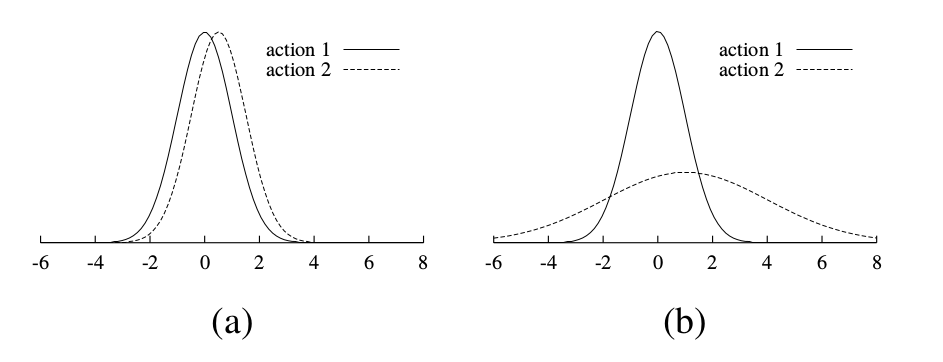
\includegraphics[width=\linewidth]{q_value_sampling.png}
 \caption{Examples of Q-value distributions of two actions for which Q-value sampling has the same exploration policy even though the payoff of exploration in (b) is higher than in (a) ~\cite{Dearden98bayesianq-learning}.}
 \label{fig:q_value_sampling}
\end{figure}
The second method of action selection is \emph{Myopic-VPI}. This method uses the distributions over the Q-values to calculate an approximation of the \emph{Value of Information} ~\cite{4082064} for each action and then selects the action that best balances exploration and exploitation according to the criterion. The idea is to balance the expected gains from exploration, in the form of improved policies, against the expected cost of doing a potentially suboptimal action. The only interesting scenarios are those where the new knowledge collected from exploration does change the agent’s policy. This can happen in two cases: 
\begin{itemize}
\item When the new knowledge shows that an action previously considered sub-optimal is revealed as the best choice (given the agent’s beliefs about other actions),
\item When the new knowledge indicates that an action that was previously considered best is actually inferior to other actions.
\end{itemize}
Based on the above logic, Dearden et al. derive closed form equations to calculate the VPI for each action, and execute the action that maximizes: 
\begin{equation}
	\mathbb{E}[Q(s,a)]+VPI(s,a).
\end{equation}
The value of exploration estimate is used as a way of boosting the desirability of different actions. When the agent is confident of the estimated Q-values, the VPI of each action is close to 0, and the agent will always choose the action with the highest expected value.
\subsubsection{Updating the Distribution}
The question of updating the distributions maintained it is complicated due to the fact that we maintain the distribution of Q-values, which are the expected total discounted reward, whereas the observations available are samples of the local reward\footnote{In this sense BQL is a distributional approach.}. For this reason, standard Bayesian results cannot be used directly. Suppose the agent is at state $s$, executes action $a$, observes next-state $s'$ and reward $r$. We would like to know the complete sequence of rewards observed from state $s'$ onward, but unfortunately this is not available. Let $R_{s'}$ be the total sum of discounted rewards collected from $s'$. If the agent will follow the optimal policy then $R_{s'}$ is distributed as $R_{s',a'}$ where $a'$ is the action with highest expected value at $s'$. Bayesian Q-Learning proposes to ways to use this distribution to substitute for the unknown future experiences.\par
The first method proposed is \emph{Moment Updating}. The idea is to sample $R_{s'}^1, \ldots, R_{s'}^n$ from the distribution of the Q-values in the next state, $R_{s',a'}$, and use these values to update $P(R_{s,a})$ with the samples $r+\gamma R_{s'}^1, \ldots, r+\gamma R_{s'}^n$. Dearden et al. show that we need just the first two moments of the distribution to perform the update, which for $n$ that tends to infinity are given by:
\begin{equation}
\label{eq:moment_updating}
\begin{split}
	& M_1= r+\gamma \mathbb{E}[R_{s'}], \\
	& M_2= r^2+2 \gamma r \mathbb{E}[R_{s'}]+ \gamma^2 \mathbb{E}[R_{s'}^2],
\end{split}
\end{equation} 
where $\mathbb{E}[R_{s'}]=\mu_0$ and $\mathbb{E}[R_{s'}^2]=\frac{\lambda+1}{\lambda} \frac{\beta}{\alpha-1}+ \mu_0^2$.
Using (~\ref{eq:moment_updating}) and standard results for normal-gamma distribution ~\cite{degroot2012probability}, Dearden et al. give the posterior $p(\mu_{s,a},\tau_{s,a} | r+\gamma R_{s'}^1, \ldots, r+\gamma R_{s'}^n) \sim NG(\mu_{0_{s,a}}',\lambda_{s,a}',\alpha_{s,a}',\beta_{s,a}')$ where:
\begin{equation}
\begin{split}
	& \mu_{0_{s,a}}'=\frac{\lambda_{s,a} \mu_{0_{s,a}} + M_1}{\lambda_{s,a}+1}, \\
	& \lambda_{s,a}'=\lambda_{s,a}+1, \\
	& \alpha_{s,a}'=\alpha_{s,a}+ \frac{1}{2}, \\
	& \beta_{s,a}'=\beta_{s,a}+\frac{1}{2}(M_2-M_1^2)+ \frac{\lambda_{s,a}(M_1-\mu_{0_{s,a}})^2}{2(\lambda_{s,a}+1)}.
\end{split}
\end{equation}
Moment updating results in a simple closed form solution, but unfortunately becomes to confident of the value of the mean $\mu_{s,a}$. This leads to low exploration values and hence to premature convergence.\par
The second update method proposed is \emph{Mixture Updating}. The method was proposed to avoid the premature convergence problem of Moment Updating. This method uses the distribution of $R_{s'}$ in a slightly different way. Let $p(\mu_{s,a},\tau_{s,a}|R)$ be the posterior distribution after observing discounted reward $R$. If we observed $R_{s'}=x$, we would have the posterior $p(\mu_{s,a},\tau_{s,a}|r+ \gamma x)$. We can capture the uncertainty of the value of $x$, by weighting this distribution with the probability $R_{s'}=x$. This way we get the following \emph{mixture distribution} :
\begin{equation}
	p^{mix}(\mu_{s,a},\tau_{s,a})=\int_{-\infty}^{\infty} p(\mu_{s,a},\tau_{s,a} |r + \gamma x) P(R_{s'}=x) d(x).
\end{equation} 
Unfortunately this distribution is no longer a normal-gamma distribution, and performing this update in every time step would result, each time, in a more complex distribution. Dearden et al. use an approximation to keep the distribution normal-gamma, but unfortunately they did not come with a closed form solution for the update. Performing Mixture update, while it leads to better and more efficient exploration, comes with higher computational effort compared to Moment Updating, as a result of the numericalcalculation of integrals needed to perform the update. \par
Finally, it is important to note that BQL does not guarantee efficient exploration. BQL guarantees convergence of the algorithm to the optimal Q-function at best, when Q-value sampling is used for action selection and Moment Update is used to update the distributions. Even though the combination of Myopic VPI and Mixture Updating gives better results in experiments, convergence is not guaranteed.
\section{Deep Exploration} \label{deep_exploration}
In the previous section we discussed a variety of provably-efficient approaches to exploration. However, these are designed for MDPs with small finite state spaces. These algorithms are not practical in complex environments where an agent must generalize to operate effectively. For this reason, large-scale applications of RL have relied upon statistically inefficient strategies for exploration ~\cite{mnih2015humanlevel} or even no exploration at all ~\cite{Tesauro:1995:TDL:203330.203343}.
Uncertainty estimates allow an agent to direct its exploration at potentially informative states and actions. In RL, directed exploration is not enough to guarantee efficiency; the exploration must also be deep. Deep exploration means exploration which is directed over multiple time steps; it can also be called ``planning to learn'' or ``far-sighted'' exploration. For exploitation, this means that an efficient agent must consider the future rewards over several time steps and not simply the myopic rewards. In exactly the same way, efficient exploration may require taking actions which are neither immediately rewarding, nor immediately informative. Several work discussed deep exploration both in model-based and model-free frameworks ~\cite{Osband:2016:GEV:3045390.3045641,Osband2017WhyIP,NIPS2013_5185,DBLP:journals/corr/OsbandR15,Osband2017DeepEV}. In this section we will review a recent algorithm that performs deep exploration in large-scale applications, Bootstrapped DQN ~\cite{DBLP:journals/corr/OsbandBPR16}.
\subsection{Bootstrapped Q Learning}
\emph{Deep neural networks} (DNN) represent the state of the art in many supervised and reinforcement learning domains ~\cite{mnih2015humanlevel}. Our objective is an exploration strategy that is statistically computationally efficient together with a DNN representation of the value function. To explore efficiently, the first step is to quantify uncertainty in value estimates so that the agent can judge potential benefits of exploratory actions. The neural network literature presents a sizable body of work on uncertainty quantification founded on parametric Bayesian inference ~\cite{Blundell:2015:WUN:3045118.3045290,Gal:2016:DBA:3045390.3045502}. One such method to represent uncertainty is the bootstrap principle.\par
The bootstrap principle is to approximate a population distribution by a sample distribution ~\cite{EfroTibs93}. In its most common form, the bootstrap takes as input a data set $D$ and an estimator $\psi$. To generate a sample from the bootstrapped distribution, a data set $\widetilde{D}$ of cardinality equal to that of $D$ is sampled uniformly with replacement from $D$. The bootstrap sample estimate is then taken to be
$\psi(\widetilde{D})$. The bootstrap is widely hailed as a great advance of 20th century
applied statistics and even comes with theoretical guarantees ~\cite{bootstrapAsymptotic}. In this section we will discuss the application of the bootstrap principle to neural networks.\par
Osband et al.~\cite{DBLP:journals/corr/OsbandBPR16} present a scalable method for generating bootstrap samples from a large and deep neural network. The architecture is shown in Figure ~\ref{fig:BDQN_Architecture}. The network consists of a shared architecture with $K$ bootstrapped ``heads'' branching off independently. Each head is trained only on its bootstrapped sub-sample of the data and represents a single bootstrap sample $\psi(\widetilde{D})$. The shared network learns a joint feature representation across all the data, which can provide significant computational advantages at the cost of lower diversity between heads. This type of bootstrap can be trained efficiently in a single \emph{forward/backward pass}.
\begin{figure}
 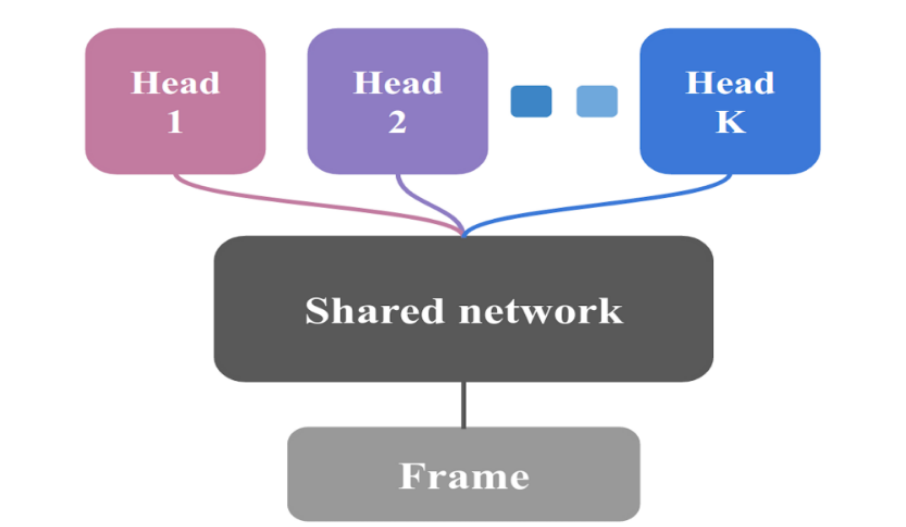
\includegraphics[width=\linewidth]{BDQN_Architecture.png}
 \caption{Network architecture in Bootstrapped DQN ~\cite{DBLP:journals/corr/OsbandBPR16}.}
 \label{fig:BDQN_Architecture}
\end{figure}
Bootstrapped DQN uses a parametrized estimate of the Q-value function, $Q(s,a;\theta)$, rather than a tabular encoding. A neural network is used to estimate this value, inspired from the architecture presented in ~\cite{mnih2015humanlevel}. The parameters $\theta$ are the weights of the neural network ~\cite{Goodfellow-et-al-2016}.\par
Bootstrapped DQN uses the modifications taken from DQN, to stabilize learning:
\begin{itemize}
\item The algorithm learns from sampled transitions from an experience buffer, rather than learning fully online,
\item The algorithm uses a target network with parameters $\theta^-$ that are copied from the learning network $\theta^- \leftarrow \theta_t$ only every $\tau$ time steps and then kept fixed in between updates.
\end{itemize}
The network update when executing action $a_t$ from state $s_t$, and observing reward $r_t$ and next state $s_{t+1}$ is :
\begin{equation}
\theta_{t+1} \leftarrow \theta_t +\alpha(y^Q_t-Q(s_t,a_t;\theta_t)) \nabla_{\theta} Q(s_t,a_t;\theta_t)),
\end{equation}
 where $\alpha$ is the learning rate and $y^Q_t$ is the target value. Bootstrapped DQN uses the target value of Double DQN ~\cite{Goodfellow-et-al-2016} to further stabilize learning. The target value $y^Q_t$ is as follows:
 \begin{equation}
 \label{eq:double_DQN_target}
 y^Q_t\leftarrow r_t+ \gamma \max_a Q(s_{t+1}, \argmax_{a} Q(s_{t+1},a;\theta_t);\theta^-).
 \end{equation}
 The Double DQN target is an elegant modification to stabilize learning. The update uses the main network to find the optimal action in the next state, but uses the value of this action from the target network. By doing this, we lower the positive bias introduced by the $\max$ operation in Q-Learning.\par
Bootstrapped DQN modifies DQN to approximate a distribution over Q-values via the bootstrap. At the start of each episode, bootstrapped DQN samples a single Q-value function from its approximate posterior. The agent then follows the policy which is optimal for that sample for the duration of the episode. The authors argue this is a natural adaptation of the Thompson sampling heuristic to RL that allows for temporally extended (or deep) exploration ~\cite{Strens00abayesian,NIPS2013_5185}. The algorithm can be implemented efficiently by building up $K \in \mathbb{N}$ bootstrapped estimates of the Q-value function in parallel as in Figure ~\ref{fig:BDQN_Architecture}. It is important to clarify that each one of these value function function heads $Q_k(s,a;\theta)$ is trained against its own target network $Q_k(s,a;\theta^-)$. This means that each $Q_1, \ldots, Q_K$ provide a temporally extended (and consistent) estimate of the value uncertainty via TD estimates. \par 
The algorithm also stores a mask, $w_1, \ldots, w_K \in \{0, 1\}$ indicating data are used to train which head. The mask, $m_t$, is a core idea of the full Bootstrapped DQN algorithm because it decides, for each value function $Q_k$, whether or not it should train upon the experience generated at step $t$. In its simplest form $m_t$ is a binary vector of length $K$, masking out or including each value function for training on that time step of experience (\ie should it receive gradients from the corresponding experience $(s_t, a_t, r_t, s_{t+1},m_t)$). The masking distribution $M$ is responsible for generating each $m_t$. For example, when $M$ yields $m_t$ whose components are independently drawn from a Bernoulli distribution with parameter 0.5 then this corresponds to the double-or-nothing bootstrap ~\cite{owen2012}. On the other hand, if $M$ yields a mask $m_t$ with all ones, then the algorithm reduces to an ensemble method.\par
Periodically, the replay buffer is played back to update the parameters of the value function network $Q$. The gradients of the $k$-th value function $Q_k$ for the $t$-th tuple in the replay buffer $B$, $g_t^k$ is:
\begin{equation}
g_t^k=m_t^k(y_t^Q-Q_k(s_t,a_t;\theta))\nabla_{\theta}Q(s_t,a_t;\theta),
\end{equation}
where $y_t^Q$ is the target value given by (~\ref{eq:double_DQN_target}). Pseudocode of the algorithm is shown in Alg.~\ref{alg:bootstrapped_dqn}.
\begin{algorithm}[H]
	\textbf{INPUT:} Value function networks $Q$ with $K$ outputs $\lbrace Q_k \rbrace_{k=1}^{K}$, Masking distribution $M$.
 \begin{algorithmic} 
 \State Let $B$ be a replay buffer storing experience
 \For{each episode}
 \State Obtain initial state $s_0$
 \State Pick a value function to act using $k \sim Uniform\lbrace1, \ldots, K\rbrace$
 \For{step $t=1, \ldots$ until end of episode}
 	\State Pick an action according to $a_t \in \argmax_a Q_k(s_t,a)$
 	\State Take action $a_t$, and observe $r_t,s_{t+1}$
 	\State Sample bootstrap mask $m_t \sim M$
 	\State Add experience ($s_t,a_t,r_t,s_{t+1},m_t)$ to replay buffer $B$
 \EndFor
 \EndFor
 \end{algorithmic}
	\caption{Bootstrapped DQN}
 \label{alg:bootstrapped_dqn}
\end{algorithm}

\section{Distributional RL} \label{distributional_rl}
In the previous chapter we reviewed the theory behind Distributional RL, and the essential importance of the value distribution. Although the distributional framework is not derived to guide exploration, it provides some relevant ideas we will reuse in our algorithm. We recall $Z(s,a)$ is the random variable denoting the total return collected by the agent starting from state $s$, executing action $a$ and then following an optimal policy, the expected value of which is $Q(s,a)$. In this section we will review two recent algorithms that belong to this class.
\subsection{Approximate Distributional Learning: C51}
In this section we discuss a recent algorithm based on the distributional Bellman optimality operator discussed in the previous chapter. C51 ~\cite{DBLP:journals/corr/BellemareDM17} models the value distribution using a discrete distribution parametrized by $N \in \mathbb{N}$ and $V_{MIN}, V_{MAX} \in \mathbb{R}$. The support of the distribution is given by a set of \emph{atoms} $\lbrace z_i= V_{MIN} + i\Delta z : 0 \leq i < N \rbrace, \Delta z= \frac{V_{MIN}-V_{MAX}}{N-1}$. The atom probabilities are given by a parametric model $\theta: \mathcal{S} \times \mathcal{A} \rightarrow R^N$. 
\begin{equation}
Z_{\theta}(s,a) =z_i \qquad w.p. 	\quad p_i(s,a)= \frac{e^{\theta_i(s,a)}}{\sum_{j=0}^{N-1}e^{\theta_j(s,a)}}.
\end{equation}
This discrete distribution is highly expressive and computationally friendly ~\cite{VanDenOord:2016:PRN:3045390.3045575}.\par
The algorithm works as follows:
\begin{itemize}
	\item From $(s,a)$, sample a transition, $r, S', A' \sim R(s,a), P(\cdot|s,a), \pi(\cdot|S')$, where $\pi$ the policy the agent follows;
	\item Compute the \emph{sample backup} given as:
	\begin{equation}
	\hat{\mathcal{T}}^\pi Z(s,a)=r+\gamma Z(S',A');
	\end{equation}
	\item Project this distribution onto the discrete distribution $z_\theta$, $\Phi \widehat{T}^\pi Z(s,a)$;
	\item Update towards projection, \ie take a KL-minimizing step.
\end{itemize}
\subsubsection{Projection step}
C51 reduces the Bellman update, discussed in the previous chapter, to multiclass classification by projecting the update $\hat{\mathcal{T}}z_\theta$ into the support of $z_{\theta}$. We recall the Bellman Operator defined in (~\ref{eq:bellman_distributional}). Figure ~\ref{fig:distributional_operator} gives an idea of this step. The framework is the same. The agent is at state $s$, executes action $a$, and observes reward $r$ and next state $s'$. We start from our prior belief about the distribution of the return in the next state, seen in Figure ~\ref{fig:distributional_operator} (a) in the figure. We want to learn from the experience collected. In Figure ~\ref{fig:distributional_operator} (b) we see how our distribution in the next state shrinks after we multiply it with the discount factor $\gamma$, and in Figure ~\ref{fig:distributional_operator} (c) we see the shifted distribution after adding the observed reward $r$. The projection step mentioned above can be seen in Figure ~\ref{fig:distributional_operator} (d). Discounting shrinks the distribution, so the target and the approximation have a disjoint support, and the KL divergence is infinite, so we cannot apply a minimization step. C51 solves this by taking every atom of the target distribution, and mapping them to its two nearest neighbors.\par
\begin{figure}
 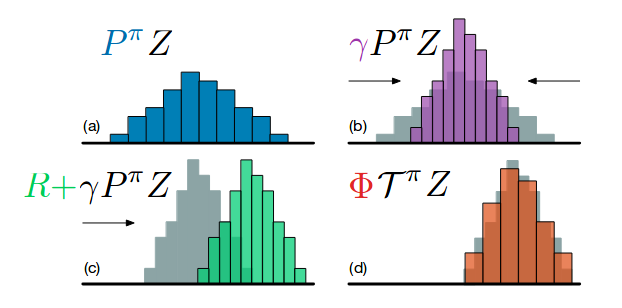
\includegraphics[width=\linewidth]{distributional_bellman_operator.png}
 \caption{Visualization of the distributional Bellman operator ~\cite{DBLP:journals/corr/BellemareDM17}.}
 \label{fig:distributional_operator}
\end{figure}
More formally, let $\pi$ be the greedy policy \wrt $\mathbb{E}[Z_\theta]$. Given a sample transition $(s,a,r,s′)$, we compute the Bellman update $\widehat{T}z_j=r+\gamma z_j$ for each atom $z_j$, then distribute its probability $p_j(s′,\pi(s′))$ to the immediate neighbours of $\widehat{T}z_j$. The $i$th component of the projected update $\Phi \widehat{T}^\pi Z(s,a)$ is:
\begin{equation}
	\Phi \widehat{T}^\pi Z(s,a)_i=\sum_{j=0}^{N-1} \left[1- \frac{\vert [\widehat{T}z_j]_{V_{MIN}}^{V_{MAX}} -z_i  \vert}{\Delta z} \right]_{0}^{1},
\end{equation}
where $[\quad]_{a}^{b}$ bounds its arguments in the range $[a,b]$. Pseudocode of the algorithm is shown in Alg. ~\ref{alg:c51}
\begin{algorithm}[H]
\begin{flushleft}
 \textbf{Input:} A transition $s_t,a_t,r_t,s_{t+1}$, $\gamma \in [0,1]$\\
 \textbf{Output:} Loss
\end{flushleft}
 \begin{algorithmic}
 \State $Q(s_{t+1},a)= \sum_{i} z_i p_i(s_{t+1},a)	\qquad \forall a$
 \State $a^* \leftarrow \argmax_a Q(s_{t+1},a)$
 \State $m_i=0, i \in 0, \cdots, N-1$
 \For{$j \in 0, \cdots, N-1$}
 		\State $\widehat{T}z_j \leftarrow [r+\gamma z_j]_{V_{MIN}}^{V_{MAX}}$
 		\State $b_j \leftarrow (\widehat{T}z_j- V_{MIN}) / \Delta z$
 		\State $l \leftarrow \lfloor b_j\rfloor, u \lceil b_j \rceil$
 		\State $m_l \leftarrow m_l+ p_j(s_{t+1},a^*)(u-b_j)$
 		\State $m_u \leftarrow m_u+ p_j(s_{t+1},a^*)(b_j-l)$
 \EndFor
 \Return $-\sum_{i} m_i \log p_i(s_t,a_t)$
 \end{algorithmic}
 \caption{$C51$ algorithm}
 \label{alg:c51}
\end{algorithm}
\subsection{Distributional Reinforcement Learning with Quantile Regression}
One of the theoretical contributions of the C51 work was a proof that the distributional Bellman operator is a contraction in a maximal form of the Wasserstein metric between probability distributions. 
Unfortunately, as noted by the authors, and further developed by Bellemare et al., the Wasserstein metric, viewed as a loss, cannot generally be minimized using stochastic gradient methods ~\cite{DBLP:journals/corr/BellemareDM17}. This negative result left open the question as to whether it is possible to devise an online distributional reinforcement learning algorithm which takes advantage of the contraction result of the Wasserstein metric. Instead, the C51 algorithm first performs a heuristic projection step, followed by the minimization of a KL divergence between projected Bellman update and prediction. C51 therefore leaves a theory-practice gap in our understanding of distributional reinforcement learning, which makes it difficult to explain the good performance of C51.\par
By appealing to the theory of \emph{quantile regression} ~\cite{koenker2005quantile}, Dabney et al. in ~\cite{DBLP:journals/corr/abs-1710-10044}, propose an algorithm, applicable in a stochastic approximation setting, which can perform distributional reinforcement learning over the Wasserstein metric. Recall that C51 approximates the distribution at each state-action pair by attaching variable (parametrized) probabilities $p_1,\ldots,p_N$ to fixed locations $z_1 \leq \ldots \leq z_N$. Quantile Regression DQN's approach is to ``transpose'' this parametrization by considering fixed probabilities but variable locations. Specifically, we take uniform weights, so that $p_i= \frac{1}{N}$ for each $i = 1,\cdots,N$. This new distribution aims to estimate \emph{quantiles} of the target distribution, hence the name \emph{quantile distribution}. Let $\mathcal{Z}_Q$ be the space of quantile distributions for a given $N$. We will denote the cumulative probabilities associated to such a distribution by $\tau_1, \ldots, \tau_N$, so that $\tau_i=\frac{i}{N}$ for $i=1, \ldots, N$.\par
Formally, let $\theta: \mathcal{S} \times \mathcal{A} \rightarrow R^N$ be some parametric model. A quantile distribution, $Z_\theta \in \mathcal{Z}_Q$ maps each state-action pair $(s,a)$ to a uniform probability distribution supported on $\lbrace \theta_i(s,a) \rbrace$. That is:
\begin{equation}
	\label{eq:quantile_distribution}
	Z_\theta(s,a)= \frac{1}{N} \sum_{i=1}^{N} \delta_{\theta_i(s,a)},
\end{equation} 
where $\delta_z$ denotes a \emph{Dirac} at $z \in \mathbb{R}$.\par
Compared to the parametrization of C51, the benefits of a parameterized quantile distribution are threefold. 
\begin{itemize}
\item We are not restricted to prespecified bounds on the support, or a uniform resolution, potentially leading to significantly more accurate predictions when the range of returns vary greatly across states;
\item This also lets us do away with the projection step present in C 51, as there are no issues of disjoint supports. This obviates the need for domain knowledge about the bounds of the return distribution when applying the algorithm to new tasks;
\item This reparametrization allows us to minimize the Wasserstein loss, without suffering from biased gradients, specifically, using quantile regression ~\cite{DBLP:journals/corr/abs-1710-10044}.
\end{itemize}
\subsubsection{The Quantile Approximation}
It is well-known that in reinforcement learning, the use of function approximation may result in instabilities in the learning process ~\cite{Tsitsiklis97ananalysis}. Specifically, the Bellman update projected onto the approximation space may no longer be a contraction. Dabney et al. analyze the distributional Bellman update, projected onto a parameterized quantile distribution, and prove that the combined operator is a contraction. \par
We are interested in quantifying the projection of an arbitrary value distribution $Z \in \mathcal{Z}$ onto $\mathcal{Z}_Q$, that is:
\begin{equation}
	\Pi_{d_1}Z= \argmin_{Z_\theta \in \mathcal{Z}_Q} d_1(Z,Z_\theta).
\end{equation}
Let $Y$ be a distribution with bounded first moment and $U$ be a uniform distribution over $N$ Diracs as in [~\ref{eq:quantile_distribution}] with support $\lbrace \theta_1, \ldots, \theta_N \rbrace$. Then the 1-Wasserstein distance is:
\begin{equation}
	d_1(Y,U)= \sum_{i=1}^{N} \int_{\tau_{i-1}}^{\tau_i} \vert F_Y^{-1}(\omega)- \theta_i \vert d \omega,
\end{equation}
where $F_Y^{1}$ is the quantile function of $Y$. We are looking for the parametrized distribution that minimizes this distance. Dabney et al. prove in ~\cite{DBLP:journals/corr/abs-1710-10044} the following: 
\begin{lemma}
	For any $\tau, \tau' \in [0,1]$ with $\tau < \tau'$ and cumulative distribution $F$ with inverse $F^{-1}$, the set of $\theta \in \mathbb{R}$ minimizing $\int_{\tau_{i-1}}^{\tau_i} \vert F_Y^{-1}(\omega)- \theta_i \vert d \omega$ is given by 
	\begin{equation*}
		\left\lbrace \theta \in \mathbb{R} \vert F(\theta)=\frac{\tau+\tau'}{2} \right\rbrace.
	\end{equation*}
	\label{lem:MinQuantileDist}
\end{lemma}
These \emph{quantile midpoints} will be denoted by $\hat{\tau}_i=\frac{\tau_{i-1}+\tau_i}{2}$ for $1 \leq i \leq N$. Therefore, by Lemma \ref{lem:MinQuantileDist}, the values for $\lbrace \theta_1,\theta_2,\ldots,\theta_N\rbrace$ that minimize $d_1(Y,U)$ are given by $\theta_i=F^{-1}_Y(\hat{\tau_i})$.\par
Dabney et al. prove that the combination of the projection implied by quantile regression with the Bellman operator is a contraction in $\infty$-Wasserstein metric, \ie the largest gap between the two c.d.fs. More formally, for any two value distributions $Z_1, Z_2 \in \mathcal{Z}$ for an MDP with countable state action spaces, 
\begin{equation}
\overline{d}_{\infty}(\Pi_{d_1} \mathcal{T}^\pi Z_1,\Pi_{d_1} \mathcal{T}^\pi Z_2) \leq \gamma \overline{d}_{\infty} (Z_1,Z_2),
\end{equation}
where $\Pi_{d_1} \mathcal{T}^\pi$ is the combined Bellman operator.\par
Following these results, Dabney et al. use the \emph{quantile regression loss}, which is an asymmetric convex loss that penalizes overestimation errors with weight $\tau$ and underestimation errors with weight $1-\tau$. More formally, for a distribution $Z$, and a given quantile $\tau$, the value of the quantile function $F_Z^{-1}(\tau)$ may be characterized as the minimizer of the quantile regression loss:
\begin{equation}
\begin{split}
\mathcal{L}_{QR}^{\tau}(\theta) & =\mathbb{E}_{\hat{Z} \sim Z}[\rho_{\tau}(\hat{Z}-\theta)], \text{where} \\
\rho_{\tau}(u) & = u(\tau- \delta_{\lbrace u<0 \rbrace}) \quad \forall u \in \mathbb{R}.
\end{split}
\label{eq:quantile_regression_loss}
\end{equation} 
More generally, we have that the minimizing values of $\lbrace \theta_1,\theta_2,\ldots,\theta_N\rbrace$ for $d_1(Z,Z_\theta)$ are those that minimize the following objective
\begin{equation*}
	\sum_{i=1}^{N} =\mathbb{E}_{\hat{Z} \sim Z}[\rho_{\tau}(\hat{Z}-\theta_i)].
\end{equation*}
This loss gives unbiased sample gradients. As a result, we can find the minimizing $\lbrace \theta_1,\theta_2,\ldots,\theta_N\rbrace$ by stochastic gradient descent. In practice the authors use the \emph{quantile Huber loss}, the asymmetric variant of the Huber loss ~\cite{huber:1964}, given by:
\begin{equation}
\mathcal{L}_k(u)=
		\begin{cases}
 \frac{1}{2}u^2 &\quad\text{if }\vert u \vert \leq k\\
 k(\vert u \vert - \frac{1}{2} k) &\quad\text{otherwise}. \\
 \end{cases}
\end{equation}
The Quantile huber loss is simply:
\begin{equation}
	\rho^k_\tau (u)=\vert \tau - \delta{\lbrace u<0 \rbrace} \vert \mathcal{L}_k(u).
\label{eq:quantile_huber_loss}
\end{equation}
\subsubsection{QRTD}
Recall the standard TD update from Chapter 1. TD allows us to update the estimated value function with a single unbiased sample following $\pi$. Quantile regression also allows us to improve the estimate of the quantile function for some target distribution, $Y(s)$, by observing samples $y \sim Y(s)$ and minimizing Equation (~\ref{eq:quantile_regression_loss}). Using these results, Dabney et al. in ~\cite{DBLP:journals/corr/abs-1710-10044} define the quantile regression temporal difference (QRTD) learning algorithm summarized by the update: 
\begin{equation}
\theta_i(s) \leftarrow \theta_i(s)+ \alpha(\hat{\tau}_1- \delta_{\lbrace r+\gamma z' < \theta_i(s) \rbrace}),
\end{equation}
where $Z_\theta$ is a quantile distribution as in (~\ref{eq:quantile_distribution}) and $\theta_i(s)$ is the estimated value of $F^{-1}_{Z^{\pi}(s)}(\hat{\tau}_i)$ in state $s$. It is important to note that this update is for each value of $\hat{\tau}_i$ and is defined for a single sample from the next state value distribution. In general it is better to draw many samples of $z′\sim Z(s′)$ and minimize the expected update. Another approach, used by the authors, is to compute the update for all pairs of $(\theta_i(s),\theta_j(s′))$.
\subsubsection{Quantile Regression DQN}
Quantile Regression DQN builds from the DQN architecture described in ~\cite{mnih2015humanlevel}. The algorithm requires two modifications to DQN. First, it uses a nearly identical neural network architecture as DQN, only changing the output layer to be of size $\vert A \vert \times N$, where $N$ is a hyper-parameter giving the number of quantile targets. Second, it replaces the Huber loss used by DQN,  with the quantile Huber loss given in Equation (~\ref{eq:quantile_huber_loss}). Pseudocode of the algorithm is given in Alg. ~\ref{alg:QRDQN}.
\begin{algorithm}[H]
\begin{flushleft}
 \textbf{Input:} A transition $s,a,r,s'$, $\gamma \in [0,1]$\\
 \textbf{Output:} Quantile Regression Loss
\end{flushleft}
 \begin{algorithmic}
 \State $Q(s',a')= \sum_{j} q_j \theta_j(s',a')	\qquad \forall a$
 \State $a^* \leftarrow \argmax_a Q(s',a)$
 \State $\mathcal{T}\theta_j \leftarrow r+ \gamma \theta_j(s',a^*), \quad \forall j$
 \State \Return $\sum_{i=1}^{N} \mathbb{E} \left[ \rho^k_{\hat{\tau}_i}(\mathcal{T}\theta_j - \theta_i(s,a)) \right]$
 \end{algorithmic}
 \caption{$QR-DQN$ algorithm}
 \label{alg:QRDQN}
\end{algorithm}